\chapter{Pravděpodobnost a inference}

\section{Úvod}

\subsection{Bayesiánská statistika}

\subsubsection{Historie}

Bayesiánská statistika je pojmenována po Thomasu Bayesovi, který v roce 1763 formuloval specifický případ Bayesovy věty. V několika svých pracích, které se datují na přelom 18. a 19. století, pak Pierre-Simon Laplace dále rozvinul Bayesiánské pojetí pravděpodobnosti. Laplace použil postupy, které jsou dnes považovány za Bayesiánské metody, k řešení řady statistických problémů. Další Bayesiánské metody pak byly představeny také pozdějšími autory.

Samotný pojem `Bayesiánská statistika' se začal používat až po roce 1950. Nicméně po většinu 20. století se Bayesiánská statistika netěšila přílišné oblibě a to z praktických důvodů. Řada Bayesiánských metod je totiž výpočetně náročná, a tak k jejich praktickému rozšíření došlo až v době nástupu výkonných počítačů.

\subsubsection{Bayesiánské vs. frekvenční pojetí pravděpodobnosti}

Bayesiánská statistika chápe pravděpodobnost jako míru našeho přesvědčení o realizaci určité události. Toto přesvědčení může vycházet z předchozích pozorování nebo může odrážet náš subjektivní názor. Tím se Bayesiánská statistika liší o tradičního frekvenčního pojetí pravděpodobnosti, v rámci kterého je pravděpodobnost založena na relativním počtu realizací dané události.

\subsubsection{Aplikace Bayesiánské statistiky}

Bayesiánské statistické metody jsou založeny na tzv. Bayesově větě, s jejíž pomocí aktualizujeme pravděpodobnost po získání nových dat. Bayesova věta tak popisuje pravděpodobnost události podmíněně jak na (a) skutečně pozorovaných datech tak na (b) našem přesvědčení. Bayesovu větu lze např. použít pro odhad parametrů pravděpodobnostního rozdělení. Protože Bayesiánské statistika interpretuje pravděpodobnost jako míru našeho přesvědčení o realizaci určité události, lze těmto parametrům přímo přiřadit pravděpodobnostní rozdělení, které toto naše přesvědčení odráží. Pravděpodobnostní rozdělení uvažovaných parametrů je pak následně možné aktualizovat na základě nově pozorovaných dat.

\subsection{Notace}

V následujícím textu budeme $\theta$ používat pro označení populačních parametrů (např. pravděpodobnost přežití pacienta), $y$ bude označovat pozorovaná data (např. počet přeživších v náhodném výběru dané velikosti), $\tilde{y}$ bude označovat neznámé avšak potenciálně pozorovatelné veličiny (např. počet pacientů, kteří přežijí po té, co se podrobili léčbě).

$\theta$ může mít charakter skaláru popř. vektoru a to podle počtu parametrů, které charakterizují danou populaci. V případě vektoru tak platí $\theta = (\theta_1, \theta_2, ..., \theta_k)$, kde $k$ je počet parametrů.

V závislosti na počtu pozorování může mít $y$ podobu jak skaláru tak vektoru. V případě vektoru platí $y = (y_1, y_2, ..., y_n)$, kde $n$ představuje počet pozorování. Pokud pro každé pozorování zaznamenáváme více než jednu charakteristiku, je $y_i$ vektorem a $y$ maticí. Z logiky věci vyplývá, že výše uvedené značení je možné analogicky aplikovat také na $\tilde{y}$.

\subsection{Zaměnitelnost}

Jedním z častých předpokladů při aplikaci Bayesiánských metod je tzv. zaměnitelnost (exchangebility). Zaměnitelnost znamená, že pravděpodobnost $p(y_1, y_2, ..., y_n)$ je invariantní vzhledem k permutacím indexů jednotlivých pozorování $y_i$. Jinými slovy např. platí $p(y_1, y_2, ..., y_n) = y(y_2, y_n, ..., y_1)$.

V praxi pak často předpokládáme, že pozorovaná data pochází jsou nejen zaměnitelná, ale že jsou také vzájemně nezávislá a že pocházejí z identického pravděpodobnostního rozdělení (tzv. iid předpoklad).

\section{Bayesiánská inference}

Statistická inference se zabývá formulováním závěrů o nepozorovaných veličinách na základě numerických dat. Příkladem takovéto nepozorované veličiny může být pravděpodobnost přežití pacienta po aplikaci nového léku. Ačkoliv tato veličina popisuje pravděpodobnost přežití v rámci celé populace pacientů, je zpravidla odhadnuta na základě náhodného výběru.


V případě Bayesiánské statistiky mají závěry ohledně parametru $\theta$ popř. nepozorovaných dat $\tilde{y}$ charakter pravděpodobnostních výroků, které jsou podmíněné pozorovanými hodnotami $y$, a v následujícím textu je budeme označovat jako $p(\theta | y)$ popř. jako $p(\tilde{y} | y)$.\footnote{Připomeňme, že $p(\cdot | \cdot)$ značí podmíněnou pravděpodobnost, zatímco $p(\cdot)$ značí marginální pravděpodobnost.}

Abychom se vyhnuli případným nejasnostem, budeme někdy pro vyjádření pravděpodobnosti určité události používat značení $Pr(\cdot)$ ve smyslu $Pr(\theta > 2) = \int_{\theta > 2} p(\theta)d \theta$.

\subsection{Bayesova věta}

Sdružená pravděpodobnost pro $\theta$ a $y$ je definována jako
\begin{equation}
p(\theta, y) = p(\theta) p(y | \theta),
\end{equation}
kde $p(\theta)$ představuje tzv. apriorní pravděpodobnostní rozdělení parametru $\theta$ (tj. pravděpodobnostní rozdělení před zohledněním pozorovaných dat $y$) a $p(y | \theta)$ představuje věrohodnostní funkci pozorovaných dat pro danou hodnotu parametru $\theta$.

S využitím Bayesovy věty lze odvodit tzv. aposteriorní pravděpodobnostní rozdělení parametru $\theta$ (tj. pravděpodobnostní rozdělení po zohlednění pozorovaných dat $y$) jako
\begin{equation}
p(\theta | y) = \frac{p(\theta, y)}{p(y)} = \frac{p(\theta)p(y | \theta)}{p(y)},
\end{equation}
kde $p(y)$  představuje pravděpodobnost realizace dat $y$ pro pravděpodobnostní model parametru $p$ definovaný apriorním pravděpodobnostním rozdělením $p(\theta)$. Platí $p(y) = \sum_{\theta} p(\theta) p(y|\theta)$ popř. $p(y) = \int_{\theta} p(\theta) p(y | \theta) d \theta$ v závislosti na tom, zda-li je $\theta$ diskrétní či spojitá veličina. 

V některých případech se aposteriorní pravděpodobnost uvádí v tzv. nenormalizované formě
\begin{equation}
p(\theta | y) \varpropto p(\theta)p(y|\theta),
\end{equation}
v rámci které jsme vynechali jmenovatel $p(y)$, protože jej lze v kontextu (1.2) chápat jako normalizační konstantu.

\subsection{Predikce}

Před tím, než vezmeme v potaz pozorovaná $y$, je pravděpodobnostní rozdělení této veličiny definováno jako
\begin{equation}
p(y) = \int p(y, \theta) d \theta = \int p(\theta) p(y | \theta) d \theta.
\end{equation}
Toto pravděpodobnostní rozdělení často nazýváme marginálním rozdělením.

Po té, co jsme pozorovali $y$, je možné analogickým způsobem zkonstruovat aposteriorní prediktivní rozdělení pro $\tilde{y}$.
\begin{equation}
p(\tilde{y} | y) = \int p(\tilde{y}, \theta | y) d \theta = \int p(\tilde{y} | \theta, y) p(\theta | y) d\theta = \int p(\tilde{y} | \theta) p(\theta|y) d\theta
\end{equation}

\subsection{Věrohodnostní funkce}

Aplikace Bayesovy věty spolu se zvoleným pravděpodobnostním modelem pro parametr $\theta$ znamená, že $y$ ovlivňuje (1.3) pouze skrze $p(y|\theta)$, což je věrohodnostní funkce, na kterou lze nahlížet jako na funkci parametru $\theta$ pro fixní data $y$. Bayesiánská inference splňuje tzv. věrohodnostní princip (likelihood principle). Ten říká, že dva pravděpodobnostní modely $p(y|\theta)$ se shodnou věrohodnostní funkcí implikují pro daná data $y$ stejnou inferenci parametru $\theta$.

\subsection{Aposteriorní pravděpodobnostní poměr}

Poměr $p(\theta | y)$ v bodech $\theta_1$ a $\theta_2$ pro daný model nazýváme aposteriorním pravděpodobnostním poměrem $\theta_1$ ku $\theta_2$
\begin{equation}
\frac{p(\theta_1 | y)}{p(\theta_2 | y)} = \frac{p(\theta_1)p(y | \theta_1) / p(y)}{p(\theta_2)p(y | \theta_2) / p(y)} = \frac{p(\theta_1)p(y | \theta_1)}{p(\theta_2)p(y | \theta_2)}.
\end{equation}
Výše uvedená rovnice říká, že tento aposteriorní pravděpodobnostní poměr je roven apriorní pravděpodobnosti vynásobené věrohodnostním poměrem $p(y | \theta_1) / p(y | \theta_2)$.

\section{Ilustrativní příklady}

\subsection{Genetika}

Muži mají jeden chromozom X a jeden chromozom Y. Ženy mají dva chromozomy X, přičemž každý z chromozomů zdědily po jednom z rodičů. Hemofilie je nemoc, která se dědí skrze chromozom X. Muž, který zdědí takto zasažený chromozom X, je nemocí zasažen. Aby hemofilií onemocněla žena, musely by být nemocí zasaženy oba její chromozomy X. Hemofilie je pro ženy smrtelná. Pravděpodobnost, že žena zdědí dva chromozomy X zasažené nemocí je však téměř zanedbatelná, protože je výskyt takto poškozených genů v populaci velmi malý.

\subsubsection{Apriorní pravděpodobnost}

Předpokládejme, že žena má otce, který hemofilií netrpí a bratra, který je nemocí zasažen. To znamená, že její matka je skrytá přenašečka  hemofilie. Žena má tak padesáti procentní pravděpodobnost, že je také skrytou přenašečkou ($\theta = 1$), a padesáti procentní pravděpodobnost, že je zcela zdravá ($\theta = 0$). Jinými slovy platí $Pr(\theta = 1) = Pr(\theta = 0) = \frac{1}{2}$.

\subsubsection{Model a data}

Dále předpokládejme, že žena má dva syny. Nechť $y_i = 1$ resp. $y_i = 0$ podle toho, zda-li je syn hemofilik či nikoliv. Vyšetření ukázalo, že oba synové jsou zdraví, tj. $y_1 = y_2 = 0$. Funkce věrohodnosti tak má podobu
\begin{equation*}
Pr(y_1 = 0, y_2 = 0 | \theta = 1) = 0.50 \cdot 0.50 = 0.25
\end{equation*}
\begin{equation*}
Pr(y_1 = 0, y_2 = 0 | \theta = 0) = 1.00 \cdot 1.00 = 1.00.
\end{equation*}

\subsubsection{Aposteriorní pravděpodobnost}

Aposteriorní pravděpodobnost, že námi uvažované žena je skrytá přenašečka, je pro $y = (y_1, y_2)$ definována jako
\begin{multline*}
Pr(\theta = 1 | y) = \frac{p(y | \theta = 1)Pr(\theta = 1)}{p(y | \theta = 1) Pr(\theta = 1) + p(y | \theta = 0)Pr(\theta = 0)} =\\
\frac{0.25 \cdot 0.50}{0.25 \cdot 0.50 + 1.00 \cdot 0.50} = \frac{0.125}{0.625} = 0.20.
\end{multline*}

Výsledek je shodný s intuicí - skutečnost, že má žena dva zdravé syny, snižuje pravděpodobnost, že je skrytá přenašečka.

\subsubsection{Přidání vícero dat}

Předpokládejme, že žena má ještě třetího syna, který je také zdráv. Celý výpočet není třeba opakovat - pouze použijeme výše uvedenou aposteriorní pravděpodobnost jako novou apriorní pravděpodobnost, čímž získáme
\begin{equation*}
Pr(\theta = 1 | y_1, y_2, y_3) = \frac{0.50 \cdot 0.20}{0.50 \cdot 0.20 + 1.00 \cdot 0.80} = 0.111.
\end{equation*}

\subsection{Překlepy}

Předpokládejme, že v anglicky psaném textu narazíme na výraz `radom''. Jaká je pravděpodobnost, že autor měl na mysli `random'' spíše než `radom''? Jestliže použijeme $y$ pro označení slova, které autor skutečně napsal a $\theta$ pro označení slova, které chtěl napsat, pak je tuto pravděpodobnost možné vyjádřit v nenormalizovaném tvaru jako
\begin{equation}
Pr(\theta | y = `radom') \varpropto p(\theta) Pr(y = `radom' | \theta).
\end{equation}

Pro zjednodušení budeme uvažovat pouze tři možnosti pro zamýšlené slovo $\theta$ a to `random'', `radon'' a `radom''. Normalizovanou aposteriorní pravděpodobnost je tak možné vyjádřit jako
\begin{equation*}
p(\theta = `random' | y = `radom') = \frac{p(\theta_1)p(y = `radom' | \theta_1)}{\sum_{j = 1}^3 p(\theta_j)p(y = `radom' | \theta_1)},
\end{equation*}
kde $\theta_1 = `random'$, $\theta_2 = `radon'$ a $\theta_3 = `radom'$. Apriorní pravděpodobnosti $p(\theta_j)$ je možné odvodit z frekvence jejich výskytu v rozsáhlém textu. Pravděpodobnosti $p(y|\theta_j)$ je pak možné získat na základě modelu popř. empirických statistik překlepů.

\subsubsection{Apriorní pravděpodobnost}

Jak již bylo zmíněno výše, apriorní pravděpodobnost je možné odvodit z frekvencí výskytu daných slov. Pro naše účely jsme tyto pravděpodobnosti získali od společnosti Google.
\begin{table}
\begin{center}
\begin{tabular}{c c}
$\theta$ & $p(\theta)$\\
\hline
`random' & $7.60 \cdot 10^{-5}$\\
`radon' & $6.05 \cdot 10^{-6}$\\ 
`radom' & $3.12 \cdot 10^{-7}$\\ 
\end{tabular}
\caption{Apriorní pravděpodobnosti pro vybraná anglická slova}
\end{center}
\end{table}
Protože uvažujeme pouze tři možné hodnoty parametru $\theta$, musíme apriorní pravděpodobnosti normalizovat konstantou, tak aby jejich součet byl rovnen jedné. Napři pro `random' je tato pravděpodobnost rovna $p(\theta = `random') = \frac{760}{760 + 60.5 + 3.12}$, viz. tabulka 1.1.

Ačkoliv je nejnižší ze všech tří, frekvence slova `radom' je na první pohled překvapivá. Jedná se však o název města, které hostí největší letecký den v Polsku.

\subsubsection{Věrohodnostní funkce}

Tabulka 1.2 shrnuje podmíněné pravděpodobnosti získané na základě modelu překlepů od společnosti Google. Je vhodné zdůraznit, že tabulka představuje věrohodnostní a nikoliv pravděpodobnostní funkci (součet pravděpodobností není roven jedné). Jedná se o podmíněné pravděpodobnosti určitého jevu (výskytu slova `radom') ze tří rozdílných pravděpodobnostních rozdělení odpovídající třem různým hodnotám neznámého parametru $\theta$. Konkrétně nám tato tabulka říká, že s 97.00\% pravděpodobností autor skutečně zamýšlel napsat slovo `radom', s 0.20\% pravděpodobností chtěl namísto `radom' napsat `random' a s téměr zanedbatelnou pravděpodobností měl na mysli slovo `radon'.

\begin{table}
\begin{center}
\begin{tabular}{c c}
$\theta$ & $p(y = `radom' | \theta)$\\
\hline
`random' & $0.001930$\\
`radon' & $0.000143$\\ 
`radom' & $0.975000$\\ 
\end{tabular}
\caption{Podmíněné pravděpodobnosti pro vybraná anglická slova}
\end{center}
\end{table}

\subsubsection{Aposteriorní pravděpodobnost}

Násobením apriorní pravděpodobnosti s věrohodností a následnou normalizací získáme aposteriorní pravděpodobnosti, které jsou zachycené v tabulce 1.3. Z této tabulky vyplývá, že slovo `radom' je s přibližně dvakrát větší pravděpodobností správné, než že se jedná o překlep ve slově `random'.

\begin{table}
\begin{center}
\begin{tabular}{c c c}
$\theta$ & $p(\theta)p(y = `radom' | \theta)$ & $p(\theta | y = `radom')$\\
\hline
`random' & $1.47 \cdot 10^{-7}$ & $0.325$\\
`radon' & $8.65 \cdot 10^{-10}$ & $0.002$\\ 
`radom' & $3.04 \cdot 10^{-7}$ & $0.673$\\
\end{tabular}
\caption{Aposteriorní pravděpodobnosti pro vybraná anglická slova}
\end{center}
\end{table}

\subsection{Americký fotbal}

\subsubsection{Bodové rozpětí}

Pro každý zápas amerického fotbalu stanovují sportovní experti tzv. bodové rozpětí. Jedná se o očekávaný počet bodů, o který favorizovaná strana v průměru porazí protivníka. Pokud je tedy např. tým A 3.50 bodový favorit nad týmem B, pak je sázka, že tým A porazí tým B o čtyři či více bodů, brána jako `férová'.

\subsubsection{Parametrický model pro rozdíl mezi výsledkem zápasu a bodovým rozpětím}

Definujme náhodnou veličinu $d = \textit{(výsledek zápasu - bodové rozpětí)}$. Obrázek 1.1a ilustruje vztah mezi bodovým rozpětím (osa $x$) a náhodnou veličinou $d$ (osa $y$) pomocí grafu pro 672 zápasů. V ideálním případě by $d$ mělo být koncentrované okolo $y = 0$. Obrázek 1.1b pak představuje histogram náhodné veličiny $d$ pro těchto 672 zápasů. V našem konkrétním případě lze použít aproximaci $d|x \sim N(0, 14^2)$, která je taktéž zanesena do obrázku 1.1b.

\begin{figure}[htp]
\centering
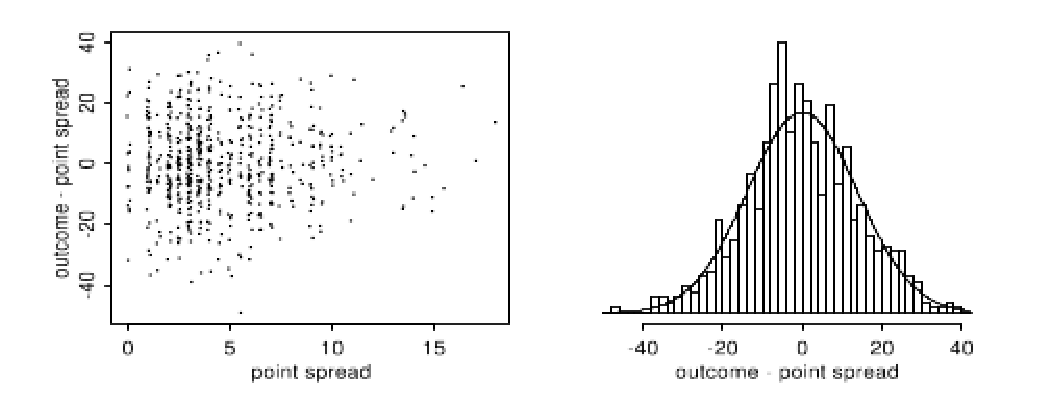
\includegraphics[scale = 0.65]{pictures/fig_1_2.eps}
\caption{(a) bodové rozpětí versus rozdíl mezi skutečným výsledkem zápasu a bodovým rozpětím; (b) histogram rozdílu mezi skutečným výsledkem zápasu a bodovým rozpětím, approximace pomocí $N(0, 14^2)$}
\label{fig_1_2}
\end{figure} 

\subsubsection{Určení pravděpodobnosti pomocí parametrického modelu}

Jestliže má $d$ normální rozdělení s nulovou střední hodnotou a je nezávislé na bodovém spreadu, pak je pravděpodobnost, že favorizovaný tým vyhraje o více než bodobý spread, rovna 50\%. Pokud bodový spread označíme náhodnou veličinou $x$, pak lze tuto pravděpodobnost vyjádřit jako
\begin{equation*}
Pr_{norm}(y > 0 | x) = Pr_{norm}(d > -x | x) = 1 - \Phi \left(- \frac{x}{14} \right).
\end{equation*}

\subsection{Párování záznamů}

Párováním záznamů rozumíme identifikaci záznamů odpovídajících stejnému objektu v různých databázích. V následujícím textu budeme tento přístup aplikovat na oficiální a testovací sčítání lidu v USA.

Párování záznamů je obvykle založeno na tom, že jsou jednotlivým polím v databázi přiřazeny váhy. S pomocí těchto vah je pak zkonstruováno skóre $y$ vyjadřující míru shody mezi dvěma záznamy. Skóre je dle zvolené metodologie vypočteno pro všechny možné páry a každý záznam je napárován se záznamem, se kterým ho pojí nejvyšší skóre.

V následujícím textu použijeme Bayesiánskou pravděpodobnost, abychom získali pravděpodobnost shody pro dané $y$ vypočteného na základě určitého rozhodovacího pravidla. Jinými slovy, pravděpodobnost shody definujeme jako funkci $y$.

\subsubsection{Empirický odhad pravděpodobnosti shody}

Přesné pravděpodobnosti lze získat pomocí tzv. směsného modelu (mixture model), který představíme v kapitole 22. Tento přístup podporuje graf 1.2, který zobrazuje histogram skóre pro skutečné a falešné shody pro 2~300 vybraných pozorování z testovacího a oficiálního sčítání lidu. Jak ilustruje graf 1.2, pravděpodobností rozdělení skutečné shody $p(y|\textit{match})$ a falešné shody $p(y|\textit{non-match})$ jsou oddělené. To znamená, že ve většině případů lze identifikovat `kandidáta'' pro napárování pouze na základě skóre.

\begin{figure}[htp]
\centering
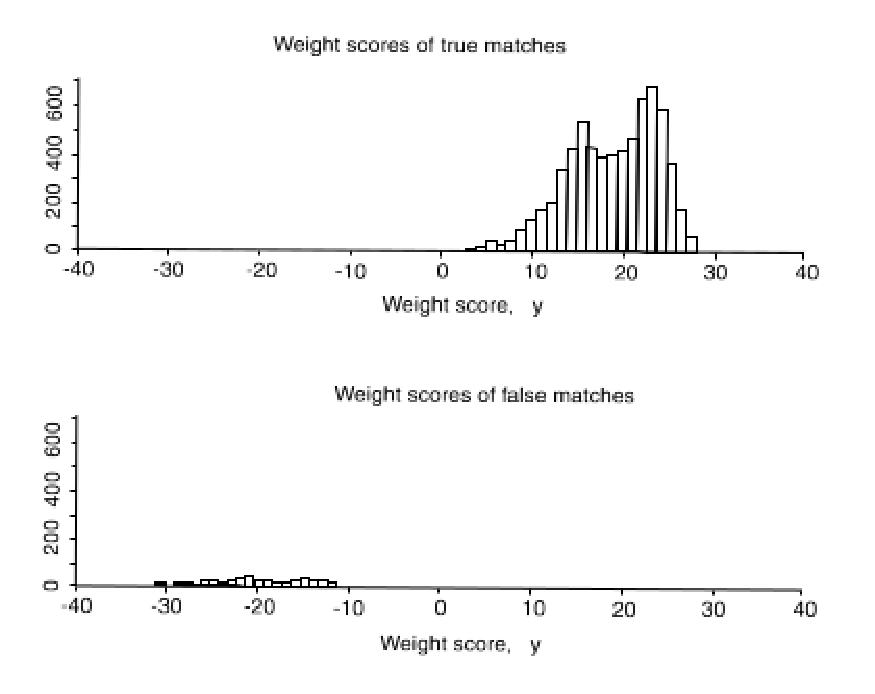
\includegraphics[scale = 0.65]{pictures/fig_1_3.eps}
\caption{Histogram skóre $y$ pro skutečné a falešné shody. Většina shod v datovém vzorku je skutečná a výše uvedená pravděpodobnostní rozdělení jsou z větší části oddělená.}
\label{fig_1_3}
\end{figure} 

Pro směsný model lze pravděpodobnostní rozdělení skóre zapsat jako
\begin{equation}
p(y) = Pr(\textit{match})p(y|\textit{match}) + Pr(\textit{non-match})p(y|\textit{non-match}).
\end{equation}

Abychom mohli použít metodu směsného modelu, zkonstruujeme křivku míry falešné shody, kdy dva záznamy jsou automaticky prohlášené za napárované, pokud jejich skóre překročí určitou hranici. Pro danou hranici je možné pomocí vztahu (1.8) odhadnout pravděpodobnost falešné shody při dosažení skóre $y$. Je zřejmé, že čím nižší je daná hranice, tím vyšší je počet automaticky napárovaných záznamů, což se však děje za cenu vyšší míry falešné shody.

\begin{figure}[htp]
\centering
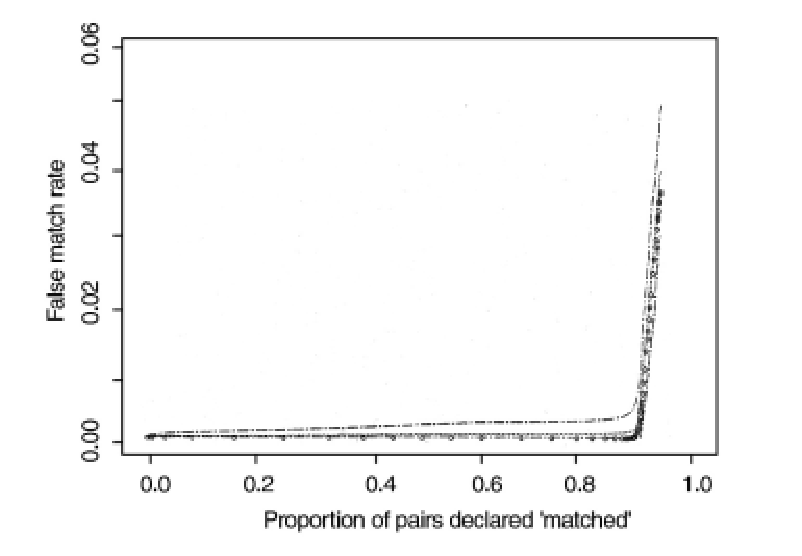
\includegraphics[scale = 0.65]{pictures/fig_1_4.eps}
\caption{Graf zobrazuje očekávanou falešnou míru shody (a 95\% interval spolehlivosti) jako podíl na celkovém počtu napárovaných záznamů podle směsného modelu. Tečkovaná čára ukazuje skutečnou míru falešné shody na pozorovaných datech.}
\label{fig_1_4}
\end{figure}

Obrázek 1.4 představuje zvětšený výřez obrázku 1.3. Z něj je patrné, že od určité hranice automaticky napárovaných záznamů rapidně narůstá míra falešné shody.

\begin{figure}[htp]
\centering
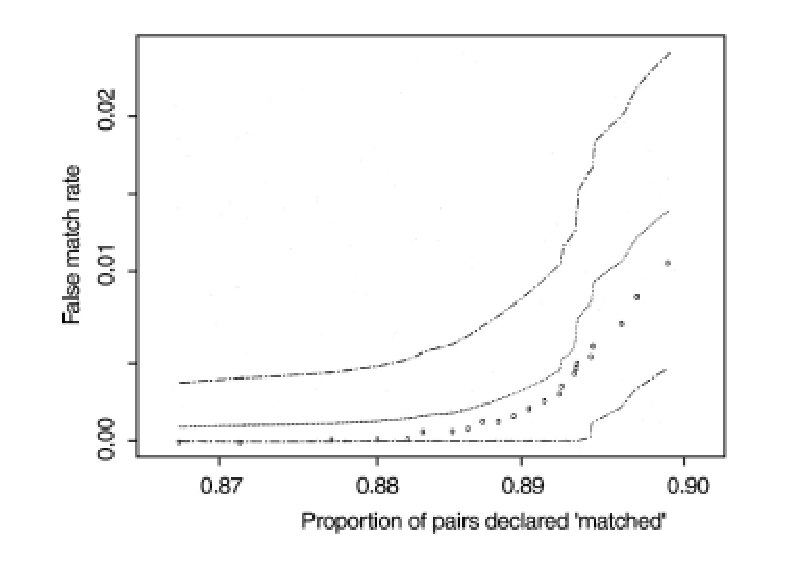
\includegraphics[scale = 0.65]{pictures/fig_1_5.eps}
\caption{Zvětšený výřez obrázku 1.3 v oblasti, pro kterou pozorujeme strmý nárůst míry falešné shody. Z obrázku je patrné, že ideálním stavem se jeví, pokud automaticky napárujeme přibližně 88\% záznamů a zbylé záznamy napárujeme ručně.}
\label{fig_1_5}
\end{figure}

\section{Několik užitečných poznatků z teorie pravděpodobnosti}

\subsection{Podmíněné pravděpodobnosti}

V Bayesiánské statistice se výpočty sdružené pravděpodobnosti $p(u, v)$ často odkazují na podmíněnou pravděpodobnost $p(u|v)$ a marginální pravděpodobnost $p(u) = \int p(u, v) dv$. Sdruženou pravděpodobnost lze totiž vyjádřit jako součin marginální a podmíněné pravděpodobnosti, tj. např. jako $p(u, v, w) = p(u | v, w) p(v | w) p(w)$. Toto rozdělení na jednotlivé součinitele značně zjednodušuje konstrukci a výpočet sdružené pravděpodobnosti.

\subsection{Hypotézy}

V zájmu zjednodušení zápisu často opomíjíme podmínění pravděpodobnosti platností určité hypotézy. Správně bychom tak např. namísto $p(\theta, y) = p(\theta) p(y | \theta)$ měli psát $p(\theta, y | H) = p(\theta | H) p(y | \theta, H)$, kde $H$ představuje soubor hypotéz a předpokladů, které definují námi uvažovaný model. V našem konkrétním příkladě má hypotéza $H$ charakter zvoleného apriorního pravděpodobnostního rozdělení parametru $\theta$.

\subsection{Střední hodnota a rozptyl}

Střední hodnotu označujeme jako $E(\cdot)$ a rozptyl jako $var(\cdot)$, kde
\begin{equation}
E(u) = \int u \cdot p(u) du, \quad var(u) = \int (u - E(u))^2 p(u) du.
\end{equation}
Pokud má $u$ podobu vektoru, je výraz pro střední hodnotu stejný a kovarianční matice, která nahrazuje rozptyl, je definována jako
\begin{equation}
var(u) = \int (u - E(u))(u - E(u))^T p(u) du.
\end{equation}

\subsection{Modelování a podmíněná pravděpodobnost}

V praxi použitelné modely často vyjadřují pravděpodobnostní rozdělení pozorovaných veličin v podmíněném popř. hierarchickém tvaru spíše než v podobě složitých nepodmíněných pravděpodobnostních rozdělení. Pro ilustraci uvažujme $y$, které představuje výšku náhodně vybraného univerzitního studenta. Marginální pravděpodobnost $p(y)$ je výsledkem kombinace dvou normálních rozdělení se střední hodnotou 160 and 175 centimetrů. Praktičtější popis pravděpodobnosti $p(y)$ by byl však založený na sdruženém rozdělení výšky a pohlaví - $p(\textit{male}) = p(\textit{female}) \approx \frac{1}{2}$ spolu s informací, že $p(y|\textit{male})$ a $p(y|\textit{female})$ jsou přibližně normálně rozdělené se střední hodnotou 175 a 160 centimetrů. Pokud není rozptyl obou normálních rozdělení příliš vysoký, pak bude výsledné pravděpodobnostní rozdělení $y$ bimodální.

\subsection{Střední hodnota a rozptyl podmíněných rozdělení}

Střední hodnotu $u$ lze vypočíst jako průměrnou střední hodnotu přes marginální rozdělení $v$, tj. jako
\begin{equation}
E(u) = E(E(u|v)).
\end{equation}
Výše uvedený vztah lze poměrně snadno odvodit.
\begin{equation}
E(u) = \int \int u \cdot p(u, v) du dv = \int \int u \cdot p(u | v) du ~ p(v) dv = \int E(u|v)p(v)dv.
\end{equation}

Odpovídající výsledek pro rozptyl se skládá ze dvou částí - ze střední hodnoty podmíněného rozptylu a z rozptylu podmíněné střední hodnoty.
\begin{equation}
var(u) = E(var(u | v)) + var(E(u | v)).
\end{equation}
Tento vztah se dá dokázat, pokud pravou stranu (1.13) rozepíšeme do tvaru
\begin{equation}
\begin{split}
E(var(u|v)) + var(E(u|v)) & = E\Big(E(u^2|v) - \big(E(u|v)\big)^2\Big) + E\big(E(u|v)\big)^2 - \Big(E\big(E(u|v)\big)\Big)^2\\
 & = E(u^2) - E\Big(\big(E(u|v)\big)^2\Big) + E\Big(\big(E(u|v)\big)^2\Big) - \Big(E(u)\Big)^2\\
 & = E(u^2) - \Big(E(u)\Big)^2\\
 & = var(u)
\end{split}
\end{equation}
Výše uvedené vztahy platí také v případě, kdy $u$ je vektor - $E(u)$ je pak vektorem a $var(u)$ maticí.

\subsection{Transformace proměnných}

Předpokládejme, že $p_u(u)$ je hustota pravděpodobnosti vektoru $u$ a že transformace $v = f(u)$ má stejný počet členů jako $u$.

Jestliže je $p_u$ diskrétní pravděpodobnostní rozdělení a $f$ je funkce, která každému $u$ přiřadí právě jedno $v$, je hustota pravděpodobnosti $v$ definována jako
\begin{equation}
p_v(v) = p_u\big(f^{-1}(v)\big).
\end{equation}
Pokud je $f$ funkce, která několika $u$ může přiřadit stejné $v$, pak
\begin{equation}
p_v(v) = \sum_{v \in f(u)} p_u\big(f^{-1}(v)\big).
\end{equation}

V případě, kdy je $p_u$ spojité a $f$ každému $u$ přiřadí právě jedno $v$, pak je sdružená hustota transformovaného vektoru $u$ dána
\begin{equation}
p_v(v) = |J| p_u(f^{-1}(v)),
\end{equation}
kde $|J|$ je Jacobián transformace $u = f^{-1}(v)$.\footnote{Jacobián $J$ je čtvercová matice parciálních derivací, jejíž $(i,j)$-tý člen je roven $\partial u_i / \partial v_j$.} Pokud může $f$ několika $u$ přiřadit stejné $v$, je $p_v(v)$ reprezentováno sumou nebo integrálem.

V případě jednorozměrné veličiny často používáme přirozený logaritmus, abychom transformovali prostor z $(0, \infty)$ na $(-\infty, \infty)$. V případě veličiny definované na otevřeném jednotkovém intervalu $(0, 1)$ pak používáme tzv. logistickou transformaci
\begin{equation}
logit(u) = \ln\Big(\frac{u}{1 - u}\Big),
\end{equation}
jejíž inverzní transformace má podobu
\begin{equation}
logit^{-1}(v) = \frac{e^v}{1 + e^v}.
\end{equation}
Další běžnou transformací je tzv. probit transformace $\Phi^{-1}(u)$, která se používá k přemapovaní prostoru $(0, 1)$ na $(-\infty, \infty)$.
